\documentclass{article}
\usepackage{v-equation}
\usepackage{minted}
\usemintedstyle{staroffice}
\vgeometry
\begin{document}

\vspace*{\fill}
\begin{center}
\begin{tikzpicture}
\tzcoor*(0, 0)(O){$O$}[b]
\tzcoor*(3, 0)(X)
\tzcoor*(-3, 0)(X')
\foreach \a in {0, 10, ..., 360}{
	\tzcoor(cos{(\a)}, 2.5*sin{(\a)})(P)
	\tznode(P){$+$}[scale=0.8]
	\tzdot(P)(7pt)
	\tzline[->, red]($(P)!0.03!(X)$)($(P)!1.3!(X)$)
	\tzline[->]($(P)!0.03!(X')$)($(P)!1.3!(X')$)
}
\tzline[<->](-5, 0)(5, 0)
\end{tikzpicture}

\end{center}
\vspace*{\fill}
\pagebreak


\vspace*{\fill}
\inputminted[tabsize=4, breaklines, linenos=true, fontsize=\small]{tex}{tikz-2.tex}
\vspace*{\fill}

\pagebreak

\vspace*{\fill}
\begin{center}
\begin{tikzpicture}
\def\l{1.5}
\tzcoor*(0, 0)(Q)(8pt)
	\tzline+[->](Q)(60:\l){$T$}[a]
	\tzline+[->](Q)(180:\l){$F_e$}[l]
	\tzline+[->](Q)(90:\l){$T\cos\theta$}[a]
	\tzline+[->](Q)(0:\l){$T\sin\theta$}[r]
	\tzline+[->](Q)(270:\l){$mg$}[b]
	\tzanglemark(60:1)(Q)(90:1){$\theta$}
	
\begin{scope}[xshift=6cm, yshift=\l cm]
\def\x{1.5}
\tzcoor*(0, 0)(O){$O$}[a]
\tzcoor*($(O)+(-\x, -3)$)(Q1){$m, q$}[bl](6pt)
\tzcoor*($(O)+(\x, -3)$)(Q2){$m, q$}[br](6pt)
	\tzline(O)(Q1){$l$}[ml]
	\tzline(O)(Q2){$l$}[mr]
	\tzline[|<->|]<0, -0.5>(Q1)(Q2){$x$}[mb]
	\tzanglemark(Q1)(O)($(O)+(0,-1)$){$\theta$}
	\tzline+[dashed](O)($(Q1)!0.5!(Q2)$)
	\tzline[dashed](Q1)($(Q1)!0.5!(Q2)$)
\end{scope}
\end{tikzpicture}

\end{center}
\vspace*{\fill}
\pagebreak


\vspace*{\fill}
\inputminted[tabsize=4, breaklines, linenos=true, fontsize=\small]{tex}{tikz-3.tex}
\vspace*{\fill}

\pagebreak

\vspace*{\fill}
\begin{center}
\begin{tikzpicture}
[thick]
\def\A{16} %angle for element
\def\r{2} %radius
\def\dr{0.1} %delta r
\def\RO{\r+\dr} %radius outer
\def\RI{\r-\dr} %radius inner
\tzcoor(0:\RO)(O') %point at right end
\tzcoor*(0, 0)(O){$q_0$}[bl](5pt)
	\foreach \a in {0, 8, ..., 352}{
		\tznode(\a:\r){$+$}[scale=0.65]
		\draw[thin](\a:\r) circle [radius=\dr];
	}
	\tzlines(O)(\A:\RO)(O)(-\A:\RO);
	\tzarc(O)(-\A:\A:\RO)
	\tzarc(O)(-\A:\A:\RI)
	\tzline[->](\A:\RO)($(\A:\RO)!2cm!(1.01*\A:\RO)$){$\Delta T$}[a]
	\tzline[->](-\A:\RO)($(-\A:\RO)!2cm!(-1.01*\A:\RO)$){$\Delta T$}[b]
	\tzline+[->](O')(2, 0){$\Delta F_e$}[r]
	\tzanglemark'(-\A:\r)(O)(\A:\r){$\d{\theta}$}(15pt)
	\tzline[<->, thick]($(O')+(0,2.5)$)($(O')+(0,-2.5)$)
	\tzarc[thick](O')(90:90+0.7*\A:1){$\d{\theta}/2$}[a=2mm, r=1mm]
	\tzarc[thick](O')(270-0.7*\A:270:1)
\end{tikzpicture}

\end{center}
\vspace*{\fill}
\pagebreak


\vspace*{\fill}
\inputminted[tabsize=4, breaklines, linenos=true, fontsize=\small]{tex}{tikz-4.tex}
\vspace*{\fill}

\end{document}